\section{Aufbau}
\label{sec:Aufbau}
Das generelle Schaltungsprinzip ist in Abbildung \ref{fig:bild3} zu sehen.\newline
Die Tiefpassschaltung lässt sich mit einem Generator antreiben, wobei hier, was
für die Durchführung wichtig ist, zwischen Sinus- und Rechteckspannung gewechselt werden kann.\newline
Parallel dazu wird ein Frequenzmesser geschaltet und an der Ausgangspannung ein Zweikanaloszilloskop angeschlossen.\newline
Außerdem kann an der Ausgangsspannung durch Umstecken auch Spannung mit einem Voltmeter gemessen werden.\newline
\begin{figure}[H]
  \centering
  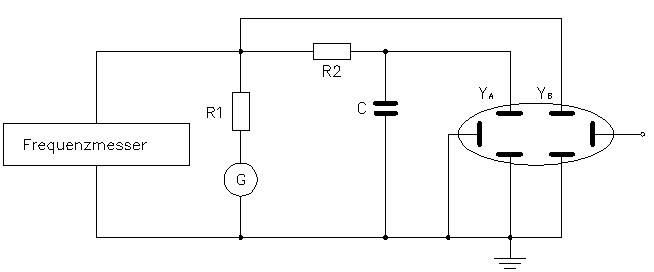
\includegraphics[scale=0.8]{bilder/bild33.png}
  \caption{Prinzipschaltung für die unterschiedlichen Messungen.}
  \label{fig:bild3}
\end{figure}
\section{Durchführung}
\label{sec:Durchführung}
Zuerst wird die Zeitkonstante des RC-Glieds bestimmt. Dazu wird mit dem Generator eine
Rechteckspannung angelegt und am Ende die Ausgangsspannung mit einem Kanal des Oszilloskops in Abhängigkeit der Zeit dargestellt.\newline
Explizit interessiert der Auf- und Entladevorgang des Kondensators; der Kondensator lädt sich auf, solange zu sehen ist, dass der Graph am Oszilloskop auf die Spannungsamplitude
steigt und er entlädt sich, wenn der Graph diesen Maximalwert verlässt und auf 0 zurück sinkt.\newline
Für eine geeignete Darstellung zur Auswertung wird die Frequenz und das Oszilloskop eingestellt, sodass sich die Spannung $U_C(t)$ um einen Faktor von 5
bis 10 ändert.\newline
Das erhaltene Bild wird mit dem Oszilloskop gespeichert.\\

Im Folgenden wird die Abhängigkeit der Spannungsamplitude am Kondensator von der Zeit bestimmt, wenn der Generator mit einer Sinusspannung
eine periodische Auslenkung vorgibt.\newline
Am Ausgang wird lediglich wieder die Spannug $U_C(t)$ gemessen.\newline
Untersucht werden mehrere Messungen in einem Frequenzbereich von $\SI{10}{Hz}$ bis $\SI{30}{kHz}$ hinweg.\\

Des Weiteren wird die Phasenverschiebung zwischen der Generator- und der Kondensatorspannung in Abhängigkeit der Frequenz bestimmt.\newline
Hierzu verwendet man unter anderem auch den zweiten Kanal des Oszilloskops, der an der Generatorspannung $U_G(t)$ angelegt wird.\newline
Ergibt sich eine Phasenverschiebung $\phi$ von $\phi > 0$, so entsteht ein Graphenverlauf wie in Abbildung \ref{fig:phase} zu sehen.\newline
\begin{figure}[H]
  \centering
  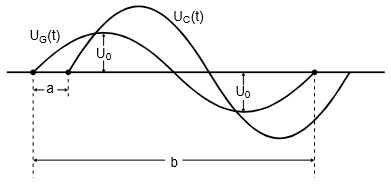
\includegraphics[scale=0.8]{bilder/bild4.png}
  \caption{Darstellung der beiden Spannungen zur Bestimmung der Phasenverschiebung\cite{anleitung}.}
  \label{fig:phase}
\end{figure}
Gemessen wird der zeitliche Abstand $a$ zwischen den beiden Nulldurchgängen. Es folgt der Vergleich mit der Schwingungsdauer $b$.\newline
Berechnet werden kann die Phasenverschiebung $\phi$ durch
\begin{equation}
\phi = \frac{a}{b} 2 \pi.
\label{eq:phi}
\end{equation}
Die Eigenschaft des Integrierens lässt sich zeigen, indem vom Generator unterschiedliche Spannungsimpulse ausgehen und sich die Spannungen am Generator $U_G(t)$ und am Kondensator $U_C(t)$
auftragen lassen. Untersucht werden die Rechtecks-, die Sinus- und die Dreiecksspannung bei hinreichend groß eingestellter Frequenz. Gemesse wurde bei einer Frequenz von $\SI{20,67}{kHz}$
